\chapter{Proposed method}

This chapter an explanation of the proposal method is described and all the
differents techniques to develop a user modeling in interactive evolutionary
computation (IEC) area such as fuzzy logic, graph-based user modeling and human-
iteraction  (gamification paradigm).

The fundamental aproach of this research is to develop a user modeling for
interactive evolutionary computation in order to increase the user participation
and to minimize the amount of evaluations for the evolutionary process in given
web-based application.

The web-based IEC applications that is used in this work is “EvoSpace framework”
mentioned in chapter 3. It is important to mention that the model it is limited
to Web-based applications and to this particular context.

In following sections explain the techniques mentioned above.


\section{Graph-based user model} 

To develop a user model, it was necessary to know the factors that are involved in
IEC system. These key factors are the following:

\begin{itemize} 
\item Individuals: The individuals are entities that create the population
of the interactive algorithm.  
\item Users: The users are the entities 
involved in the evaluation of individuals generated in the interactive genetic
algorithm replacing the fitness function.
\item User-Interaction: It is the platform where users make their evaluations in an 
easy and fast way.
\item User activity: They are the set of actions that the user performs in the application. 
\end{itemize}


Knowing these factors a graph-based user modeling is developed 

Where the vertices are defined by set of users, individuals, and
collections. The Edges are define by set of relationships as LIKES, KNOWS, HAS, PARENT that represents the relationships between the vertices as seen in \ref{fig:graph}. In this sense a formal definition is given by following definition.


\begin{equation*}\label{eq:graphRelDef} 
\displaystyle 
\begin{split} 
V &= \{[u_1,u_2,u_3,...,u_n],[i_1,i_2,i_3,...,i_n],[c_1,c_2,c_3,...,c_n]\},\\ 
E&= \{[l_1,l_2,l_3,..,l_n],[p_1,p_2,p_3,...,p_n],[h_1,h_2,h_3,...,h_n],[k_1,k_2,k_3,...,k_n]\}\\ 
\end{split} 
\end{equation*} 

Where $V$ is a set of vertices and $u$ represents users, $i$ represents
individuals, and $c$ represents collections. Also $E$ is a set of edges where
$l$ represents the relationship "LIKES" ,$p$ represents the relationship
"PARENT", $h$ represents the relationship "HAS" and finally $k$ that represents
the relationship "KNOWS".

In each vertex is necessary to store some knowledge about them, for instance in
the vertex $u$ has the properties identifier, name, creation date and name type.
Where identifier is a unique number to identifies the user, creation date is a
property where the vertex was created and name type is label for classify the
vertex in this case a “Person” label is apply. Also for vertex $i$ has the
properties identifier,  creation date, name type. Where identifier is a unique
alphanumerical value  that identify the individual, creation date is when this
vertex is created and finally name type that is a label of classify the vertex
in this case a “Individual” label is apply. Now for the  $c$ vertex has the same
properties as the $u$ vertex for their definitions of identifier and creation
date, the difference is the name type property that is a table for classify the
vertex in this case a “Collection” label is apply.

It is important to mention that the application for this research is using
EvoSpace-Interactive through the EvoSpace framework. Also another thing to
mention  is the generation of the initial individual population process in
EvoSpace is gather to transform this individuals in vertices or nodes in order
to  be ready for the evaluations of the users.
 
This user modeling is created when the users starts to interact whith the
application. In order to a user start evaluating individuals  in the application
an essential process is required. These process is that the user has a
“Facebook” account. Ones the user is access he/she can starts to interact with
the different tasks presented by the application. Thus the user can evaluate,
generate collection of individuals and also views friends individuals
collections presented in the human-interacting interface, bring us the creation
of the graph-based user modeling.


\begin{figure*}
\captionsetup{justification=centering,margin=2cm}
\centering
\setlength\fboxsep{0pt}
\setlength\fboxrule{0.7pt}
\fbox{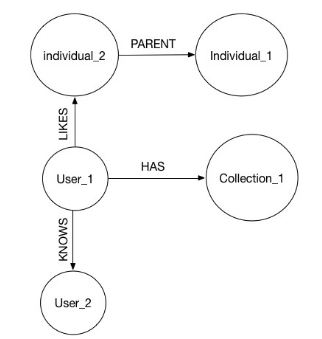
\includegraphics[width=10cm,height=10cm,keepaspectratio]{img/graph.png}}
\caption{GRAPH REPRESENTATION.}
\label{fig:graph}       
\end{figure*}


\section{Interface}
In particular, we shall explain how it was necessary to create an application called “EvoDrawings” to improve the way users interact “collaborate” with an interactive evolutionary computing system. One important class of this application is the user interface, which is the model we will explain in this chapter.

EvoDrawings is a web-based application of interactive evolutionary computing system. In these days when social media platforms has become the perfect tool for masses to exchange information/ideas, interests and creations, EvoDrawings include as a common requirement to the users to have an account of the social platform “Facebook” to have access to the application and consequently participate in it.

The main point to have users logged in the application is that they can evaluate individuals that are formed as a digital paint composed for a single chromosome of nine positions of real numbers.
Each post of the chromosome represents some figure, color, performing behavior, etc. In figure \ref{fig:graph} we can observe a chromosome composed of 15 elements from a digital paint. Once the individual is shown, the users can proceed to evaluate the individual subjectively. This means that according to the user's preferences the user can print his taste in all the evaluations.
The evaluation method consists of giving the desired rating through an interactive visual component of five stars. The interactive visual component allows the user to select from one to five stars to evaluate the individual, having the one star as a slightly liking rate and the five stars like a total satisfaction rate. 
The application enables the user to visualize his social network and the personal evaluation of the users from his social net. In addition to this, the users can create collections with the main goal to allow the users to stock the more pleasing digital paints based on his preferences. 
Also, the user interface contains a section called “About” where the application explains to users in a general way what the application is all about.
For users interact with the interactive evolutionary computation system  it was necessary to develop an application which is called “EvoDrawings”. In this point an explanation of the human-computer interface that was used  is given. 

EvoDrawing It is a Web-based application of interactive evolutionary computation. In this application users need an account of the social network platform in particular "Facebook" to access the application and consequently participate. Once users access can evaluate individuals presented as a digital painting that is composed of a chromosome, where its representation is a vector of real numbers of fifteen positions. Each position in the  chromosome  represents some kind of behavior, for instance  the type of figure, movement, color, and so on. Figure \ref{fig:graph} chromosome composed of 15 items represent a digital painting is displayed. Once the individual is shown, users come to evaluate in a subjectively way. This means that according to the likes, preferences, and so on., users conduct their evaluations. 

To evaluate individuals, users are presented with a component of visual interaction based on star ratings. This visual component is from one star to five star where  a star means that the user does not like much the painting and five means total satisfaction. Within the applications users can create collections in order to store paintings are met their expectations, in other words having a grate like for them. 

Users can view their friends who are using the application as well as see what level of experience (participation) in a leaderboard. This in order to motivate them to evaluate more Individuals and consequently Increase Their participation Within the application.

In the interface there is a section of "About" where he explains to users in a general way that addresses the application of EvoDrawigns. In the interface there is a section of "About" which explains to the  users in a breve way what the application is all about. This human-computer web-based interface can be seen in figure x.



\begin{figure*}
\captionsetup{justification=centering,margin=2cm}
\centering
\setlength\fboxsep{0pt}
\setlength\fboxrule{0.7pt}
\fbox{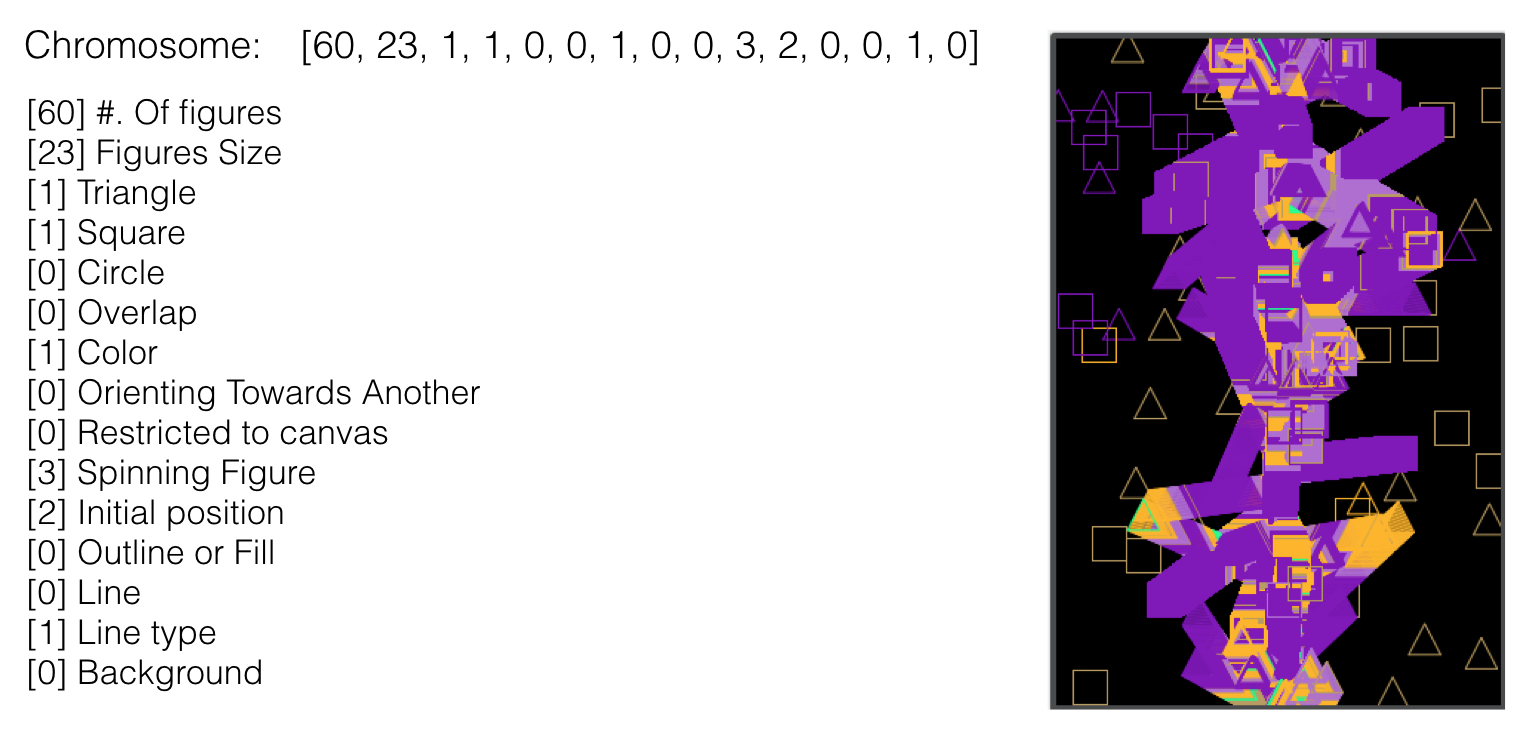
\includegraphics[width=10cm,height=10cm,keepaspectratio]{img/chromosome.png}}
\caption{CHROMOSOME REPRESENTATION.}
\label{fig:chromosome}       
\end{figure*}



We can find the vertices that are defined by the users, individuals, and collections as we can observe in figure 1. The users has the following properties:

\section{User activity}
The user activity is not so different from how the graph is formed, with the difference that the information generated is formed using the standard specified by "JSON activity stream 1.0," which is stored in the engine database NoSQL "Redis ."

An activity consists of 4 elements: an actor, a verb, an object and a target. The activity generates the history of a user and performs an action on an object. For example - "Christian likes the individual 3" or "Mario created a collection". In most cases, the components will be explicit, but may also be implicit.

The primary goal of this specification is to provide sufficient metadata about the activity, to help the consumer of these data to present the information to the user, in a straightforward and user-friendly format. This involves building simple sentences on the activity that is happening, as well as the visual representation of the activity.

So far, we can say that an "Activity Stream" is a collection of one or more activities of an individual (user).
This specification does not define the relations between the activity within the collection, therefore remains to the interpretation of the user who implements it.

\section{Database for interactive evolutionary computation}
Our data store for interactive evolutionary computation consists of two databases, as figure \ref{fig:databases} shown. On one hand one  data base  engine for EvoSpace uses Redis database already explained in Chapter x.  This database contains the structure of individual-user data, where every user participation is store, for instance the fitness of the individual, the  user identifier, the representation of the chromosome, and so on. It is necessary to have this information because is used in the fuzzy inference block , which is explained later in this chapter. 
On the other hand there is a relational database, where basic user information is stored, such as a user ID, your email, user session. Also this database  stores everything needed to meet the requirements process login "Facebook". It also contains the structure for storing collections as we can see in Figure x.

\begin{figure*}
\captionsetup{justification=centering,margin=2cm}
\centering
\setlength\fboxsep{0pt}
\setlength\fboxrule{0.7pt}
\fbox{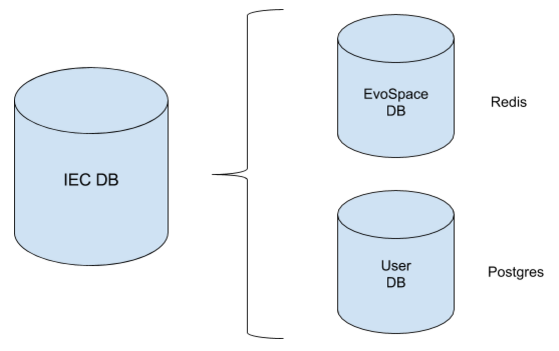
\includegraphics[width=10cm,height=10cm,keepaspectratio]{img/databases.png}}
\caption{DATABASES FOR IEC.}
\label{fig:databases}       
\end{figure*}



The database for interactive evolutionary computation consists of two databases, as we observe in figure X. In one hand we have the EvoSpace database that uses Redis database engine that is already explained in Chapter X section X.

This database contains the structure of individual user data, where every user participation is being stored as well as the fitness of the individual, the user identifier, the representation of the chromosome, etc. 

It is necessary to have this information because it is used for fuzzy inference block, which is explained in another chapter. On the other hand, we have a relational database, where basic user information is stored, such the ID, the email, the session, etc. This database also stores everything needed to meet the requirements of login for "Facebook". One important additional information is that contains the structure for storing collections as we can see in Figure X.

\section{Fuzzy Inference}
In this chapter, we will focus on the explanation of fuzzy inference block. This block uses fuzzy inference to acquire a parameter having the weight function to adjust the participation in interactive evolutionary computing applications. This parameter is used in the decision block which will be explained later in this chapter. Additionally, the parameter is also acquired from the information generated in different databases.

The fuzzy inference system is Mamdani type and is composed of three inputs and one output. Where entries are defined by the preference variable that is also composed of three functions of triangular membership; these features are called low, medium, high, and have ranged from 1 to 5. This range is given by the preference that the user assigns to the individual at the time of assessment.

We also consider the input variable called "experience" and it is defined by three functions of triangular membership under the name of low, medium and high in a range of 1 to 100. The range of this variable are acquired from the activities that the user performs in the application, and empirically with each activity, a score is assigned. For example, if the user makes a login, a three-point score is assigned, as well if the user evaluates an individual, a two-point score is assigned, all the activities has a score punctuation and also the user has a score limit of one hundred points.

The third variable which is called “ranking” it is also defined by three triangular membership functions with the name of low, medium, high, in a range of 1 to 30. This range is defined by a ranking process as well as is also performed in video games; the range is adjusted according to the user participation.

This involvement is acquired from all the cardinality of the graph that the user has and passes through the logarithmic equation X that calculates the value of ranking. Finally, the exit "fuzzyrate" is in a range of 1 to 100 defined by three triangular membership functions with the name of bad, normal and good. In figure ref{fig:Fuzzy} shows this fuzzy inference system.

Falta imagen aqui

\begin{enumerate} 

\item \textit{If \textbf{preference} is low and 
\textbf{experience} is low and \textbf{ranking} is low then \textbf{fuzzy-rate} is bad.}
\item \textit{If \textbf{preference} is low and 
\textbf{experience} is low and \textbf{ranking} is mid then \textbf{fuzzy-rate} is bad.}
\item \textit{If \textbf{preference} is low and 
\textbf{experience} is low and \textbf{ranking} is high then \textbf{fuzzy-rate} is bad.}
\item \textit{If \textbf{preference} is low and 
\textbf{experience} is mid and \textbf{ranking} is low then \textbf{fuzzy-rate} is bad.}
\item \textit{If \textbf{preference} is low and 
\textbf{experience} is mid and \textbf{ranking} is mid then \textbf{fuzzy-rate} is bad.}
\item \textit{If \textbf{preference} is low and 
\textbf{experience} is mid and \textbf{ranking} is high then \textbf{fuzzy-rate} is normal.}
\item \textit{If \textbf{preference} is low and 
\textbf{experience} is high and \textbf{ranking} is low then \textbf{fuzzy-rate} is normal.}
\item \textit{If \textbf{preference} is low and 
\textbf{experience} is high and \textbf{ranking} is mid then \textbf{fuzzy-rate} is normal.}
\item \textit{If \textbf{preference} is low and 
\textbf{experience} is high and \textbf{ranking} is high then \textbf{fuzzy-rate} is normal.}
\item \textit{If \textbf{preference} is mid and 
\textbf{experience} is low and \textbf{ranking} is low then \textbf{fuzzy-rate} is bad.}
\item \textit{If \textbf{preference} is mid and 
\textbf{experience} is low and \textbf{ranking} is mid then \textbf{fuzzy-rate} is normal.}
\item \textit{If \textbf{preference} is mid and 
\textbf{experience} is low and \textbf{ranking} is high then \textbf{fuzzy-rate} is normal.}
\item \textit{If \textbf{preference} is mid and 
\textbf{experience} is mid and \textbf{ranking} is low then \textbf{fuzzy-rate} is normal.}
\item \textit{If \textbf{preference} is mid and 
\textbf{experience} is mid and \textbf{ranking} is mid then \textbf{fuzzy-rate} is normal.}
\item \textit{If \textbf{preference} is mid and 
\textbf{experience} is mid and \textbf{ranking} is high then \textbf{fuzzy-rate} is normal.}
\item \textit{If \textbf{preference} is mid and 
\textbf{experience} is high and \textbf{ranking} is low then \textbf{fuzzy-rate} is normal.}
\item \textit{If \textbf{preference} is mid and 
\textbf{experience} is high and \textbf{ranking} is mid then \textbf{fuzzy-rate} is normal.}
\item \textit{If \textbf{preference} is mid and 
\textbf{experience} is high and \textbf{ranking} is high then \textbf{fuzzy-rate} is normal.}
\item \textit{If \textbf{preference} is high and 
\textbf{experience} is low and \textbf{ranking} is low then \textbf{fuzzy-rate} is normal.}\
\item \textit{If \textbf{preference} is high and 
\textbf{experience} is low and \textbf{ranking} is mid then \textbf{fuzzy-rate} is normal.}\
\item \textit{If \textbf{preference} is high and 
\textbf{experience} is low and \textbf{ranking} is high then \textbf{fuzzy-rate} is good.}\
\item \textit{If \textbf{preference} is high and 
\textbf{experience} is mid and \textbf{ranking} is low then \textbf{fuzzy-rate} is normal.}\
\item \textit{If \textbf{preference} is high and 
\textbf{experience} is mid and \textbf{ranking} is mid then \textbf{fuzzy-rate} is normal.}\
\item \textit{If \textbf{preference} is high and 
\textbf{experience} is mid and \textbf{ranking} is high then \textbf{fuzzy-rate} is good.}\
\item \textit{If \textbf{preference} is high and 
\textbf{experience} is high and \textbf{ranking} is low then \textbf{fuzzy-rate} is good.}\
\item \textit{If \textbf{preference} is high and 
\textbf{experience} is high and \textbf{ranking} is mid then \textbf{fuzzy-rate} is good.}\
\item \textit{If \textbf{preference} is high and 
\textbf{experience} is high and \textbf{ranking} is high then \textbf{fuzzy-rate} is good.}\

\end{enumerate} 

\begin{figure*}
\captionsetup{justification=centering,margin=2cm}
\centering
\setlength\fboxsep{0pt}
\setlength\fboxrule{0.7pt}
\fbox{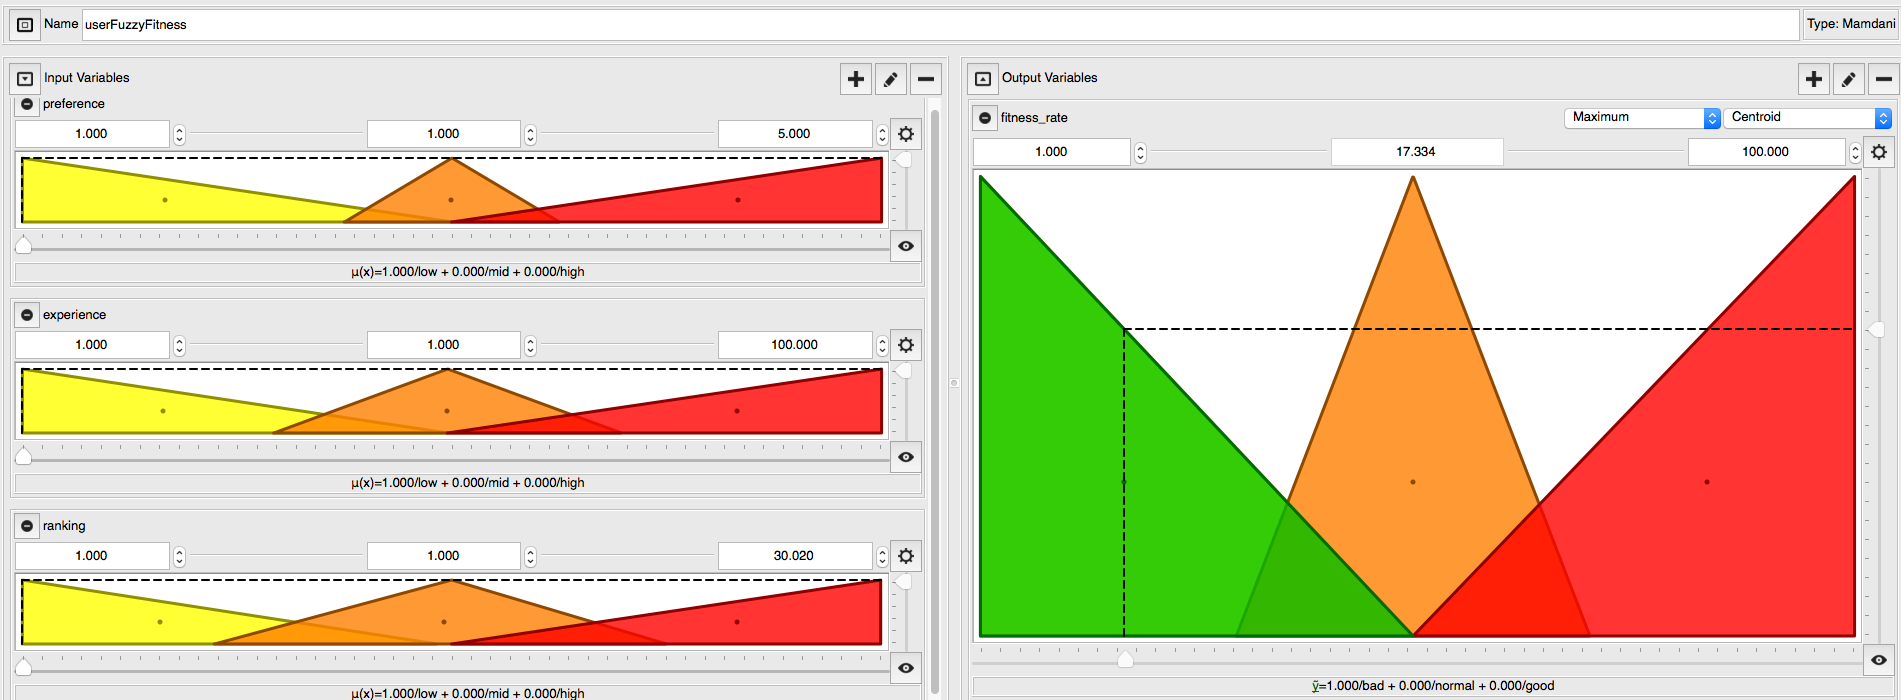
\includegraphics[width=10cm,height=15cm,keepaspectratio]{img/fuzzySys.png}}
\caption{Fuzzy Inference System.}
\label{fig:Fuzzy}       
\end{figure*}


\section{Decision Making}
The decision block it is defined by equation \ref{eq:fuzzyfitness} representing the value of fitness that takes the individual to be evaluated by the user, as well as everything else that makes in the application.

\begin{equation}\label{eq:fuzzyfitness}
\displaystyle f(ff)=\frac{\sum_{i=0}^{n}x_{i}f(y_{i})}{\sum_{i=0}^{n}f(y_{i})}
\end{equation}

Where  $ff$ represents the fuzzy fitness function for all users who have evaluated an individual of the population in particular.
Likewise $x$ represents the range that a user assigned to the individual according to their preferences, likes, and so on. The function $f(y_i)$ represents the fuzzy inference and is defined by the equation \ref{eq:fuzzyInference}.

\begin{equation}\label{eq:fuzzyInference}
\displaystyle f(y_i)= fr(x, e, r)
\end{equation}

Where $x$ is still the range that users assigned to a particular individual. The variable $e$represents the user experience, which is a function that is defined in equation \ref{eq:fuzzyInference}.

\begin{equation}\label{eq:userEperience}
\displaystyle f(e) = \sum_{i=0}^{n}l_{i}j_{i}s_{i}s_{i}
\end{equation}

Where $i$ represents user activity. The variable $l$ represents the taste generated of the verb "like" from the user activity stream.
The variable  $j$ represents the access that like the variable  is obtained from the verb "join" from the user activity stream. The variables $s, o$ are represented by the verbs "save" and "open" from the user activity stream.

\begin{equation}\label{eq:scale}
\displaystyle s =\frac{levels}{log_{2}fp}
\end{equation}

In equation \ref{eq:fuzzyInference}, we can find the variable $r$ as the last parameter of the funtion and represents a ranking of the user; this variable is defined by a logarithmic scale where intervenes our graph-base user modeling  and is defined by Equation \ref{eq:scale}.

In equation \ref{eq:scale}, the variable $s$ represents the scale and $levels$ represents the highest level that the users can have. The variable $fp$ represents the final points, which are the maximum points that a particular user can have.

In order to acquire the user's ranking level , a floor function  is calculated, the main point of this is to increase the difficulty for the high ranked users to level up. In other words the expert users needs to have more participation if they want to increse their level ranking. This function is defined by equation \ref{eq:floorf}.

\begin{equation}\label{eq:floorf}
\displaystyle rl=\lfloor(s)(log_2pf)\rfloor
\end{equation}

Where $rl$ represents the ranking lavel, $s$ represents the scale and  are all the participations  that the user has made. These participations represents the degree that the user has within his own graph and is defined by the vicinity of its vertex  that is given by the adjacent vertices to $u$, defined in Equation \ref{eq:neighbors}.

\begin{equation}\label{eq:neighbors}
\displaystyle N(u)={\{y\in V_{G}|\{u,y}\in E_{G}\}
\end{equation}

In this case the degree of the vertex $u$ is the number of neighbors of: 

\begin{equation}\label{eq:degree}
\displaystyle g(u)=|N(x)|
\end{equation}

we represent this participation as we can see in figure x.









